\documentclass[a4paper,11pt]{report}

% -- TOC --
\usepackage[nottoc,section,numbib]{tocbibind}
\usepackage[titles]{tocloft}

% -- Typography --
\usepackage[utf8]{inputenc}
\usepackage{microtype}

% -- Fonts --
%\usepackage{charter}
%\usepackage{palatino}

% -- Math --
\usepackage{amsmath}

% -- Tables --
\usepackage{booktabs}

% -- Graphics --
\usepackage{pgfplots}

% -- Misc. --
\usepackage{hyperref}
\usepackage{color}
\usepackage{array}
\usepackage{url}

\title{Internal Assessment\\
    Replication of Loftus and Palmer (1974)}
\author{Siddharth Mahendraker\\
    Psychology HL\\}

\begin{document}
\maketitle

\begin{abstract}
This paper investigates the influence of leading questions on memory by
replicating the famous study conducted by Loftus and Palmer in 1974. After
watching a video of a car crash, participants are asked a leading question
wherein the verb describing the collision is controlled (“smashed”, “hit”).
The question asks the participants to estimate the speed of the collision
(and hence recall it from memory). The results indicate that the schemata
associates with the verb in the leading question influence the recall of
the event, and result in an inaccurate reconstruction of the memory. More
specifically, mild verbs such as “hit” resulted in lower speed estimates,
while more intense verbs such as “smashed” elicited higher speed estimates.
As in the original study, these results support the conclusion that leading
question do indeed have a significant influence on memory, specifically
recall, as they introduce new information which may trigger certain schemata
and hence interfere with memory retrieval.
\end{abstract}

% -- Bookkeeping
\setcounter{secnumdepth}{3}
\renewcommand{\thesection}{\arabic{section}}
\renewcommand{\cftsecfont}{\bfseries}
\settocbibname{References}
\setlength\cftbeforesecskip{3pt}
\setlength\cftbeforesubsecskip{3pt}

% -- Easier footnotes
\newcounter{fn}
\newcommand{\fnt}[1]{%
\addtocounter{fn}{1}%
\footnote[\value{fn}]{#1}}

% -- ToC --
\setcounter{page}{1}
\pagenumbering{roman}
\tableofcontents
\clearpage
\setcounter{page}{1}
\pagenumbering{arabic}

\section{Introduction}

Memory is the cognitive process which deals with storing and retrieving
information. Unlike a computer’s hard drive, it is well known that human memory
does not store information exactly. In fact, we have all experienced the
failure of our memory at some time or another; we have all endured the
experience of being unable to remember the details of significant events or
experiences. In this sense, memory (particularly the retrieval of information
in our memory) is inherently unreliable; it suffers from inaccuracy and is
subject to change over time.

The unreliable nature of memory was first rigorously investigate by Bartlett in
1932 \cite{bartlett}. He suggested that instead of recording information
exactly, memory encodes information by processing it using mental structures
called schemes. He conjectured that schemes provide a framework for organizing
incoming information based on prior cultural and experiential knowledge. Thus
the memory process was not based on recording information verbatim, but rather
processing information using prior information as a “guide”. Bartlett further
hypothesized that the unreliability of memory stemmed from the its reliance on
schemes to process information; particularly, he suggested that when
information was retrieved from memory, it is distorted after having been
processed using personal and cultural schemes.

To test his theory of memory, Bartlett conducted a study wherein British
participants were asked to serially reproduce a traditional Aboriginal story
containing many elements specific to Aboriginal culture and storytelling. He
found that the participants’ retelling of the story changed significantly the
more it was told. More interestingly, he found that the participants’
recollection of the story changed to suit their personal and cultural schemes:
the story became shorter and details deemed insignificant to the Englishmen
were removed and replaced with details from their own cultures. These results
supported Bartlett’s hypothesis. Indeed, the results suggest that memory was
distorted by processing via cultural and personal schemes. Bartlett’s theory of
memory is called the reconstructive theory of memory, because it is based on
the idea that memory is a consequence of processing information using prior
knowledge (in the form of schemes). Bartlett’s theory of reconstructive memory
spurred significant interest and was subsequently supported by multiple
empirical studies. Today, it is a widely accepted theory of memory.

Based on the theory of reconstructive memory, Loftus and Palmer wanted to know
whether the use of leading questions influenced the reliability of information
recall; particularly in the context of courtroom examinations. Leading
questions are questions which suggest a particular answer, for example, the
question “Did you see the broken sign?” suggests that a broken sign exists. A
non-leading version of this question could be “Did you see a broken sign?”.
Loftus and Palmer conjectured that the information embedded in leading
questions could evoke processing by particular schemes during recall, and thus
interfere with recall.

In 1974, the duo conducted a study to investigate this hypothesis \cite{lap}.
In their study, participants were shown video footage of two cars colliding,
and were asked a leading question regarding the speed at which the cars
collided. The leading question contained a control verb which gave information
about the incident (“contacted”, “hit”, “smashed”). The researchers found that
the control verb had a significant influence on speed estimates. Specifically,
more dramatic verbs such as “smashed” elicited high speed estimates, while
milder verbs such as “contacted” elicited low speed estimates. These results
support the researchers’ hypothesis. The results suggest that the speed
information embedded in the control verb evoked particular schemes associated
with words such as “smashed” and “contacted”, and subsequently interfered with
recall to increase or decrease speed estimates, respectively. In the context of
courtroom examination, this meant leading question had a significant impact on
the reliability of witnesses’ answers.

In this paper, we attempt to replicate the study conducted by Loftus and
Palmer. The aim of this study is to investigate how the use of specific control
verbs in leading questions (IV) influences the reliability of recall, using the
influence of leading questions on speed estimates as a proxy (DV). We
hypothesize that the information embedded in the control verb will interfere
with the recall of information in accordance with the scheme evoked by the verb
in the leading question, and thus reduce reliability. More specifically, we
hypothesize that the use of dramatic control verbs, such as “smashed”, will
elicit overly high speed estimates, while mild control verbs, such as
“contacted”, will elicit overly low speed estimates. Otherwise, our null
hypothesis is that information embedded in leading questions will not interfere
whatsoever with the reliability of recall, more specifically, that the control
verb will have no influence on the magnitude of the speed estimates. These
hypotheses are clearly justified by the prior literature; they follow directly
from the results of Loftus and Palmer and the ideas of Bartlett.

\section{Method}

\subsection{Apparatus}

\begin{itemize}
\item Consent and briefing form
\item Debriefing form
\item Video of car crash
\item Questionnaire with the “contacted” control verb
\item Questionnaire with the “smashed” control verb
\item Laptop computer
\item Pencils
\item Eraser
\end{itemize}

See the appendix for a detailed overview of the various forms.

\subsection{Procedure}

Participants were greeted and asked to read and sign a consent form which also
briefed them on the general outline of the experiment. The specific aim of the
experiment was not mentioned; rather participants were simply told that they
would witness a car crash and answer a questionnaire. See appendix section XX
for an overview of the form given. After consenting and reading the briefing,
participants were verbally reminded their rights as participants.

The participants were then led into a quiet classroom (or hallway), and seated
in front of a table. On the table was a laptop, open to the first frame of the
car crash video (appendix YY), an overturned questionnaire, and a pencil. The
questionnaire was selected randomly from a shuffled set of questionnaires. The
participants were asked to play the video once and complete the questionnaire
when the examiner left the premise, and then inform the examiner when they had
finished. See appendix section YY for an overview of the questionnaire.

After they indicated they were finished filling out the questionnaire,
participants were verbally de-briefed and given a debrief form which explained
the objective of the experiment in greater detail. The video on the laptop was
then reset in preparation for the next participant. See appendix section ZZ for
an overview of the debriefing form.

\subsection{Design}

The experiment was designed as an independent measures laboratory experiment.
This enabled us to establish a controlled environment and establish a clear
cause and effect relationship between the IV (the control verb in the question)
and the DV (the speed estimate). There were two experimental groups comprised
of 10 students each: the group which received the “smashed” control verb in
their questionnaire, and the group which received the “contacted” control verb
in their questionnaire. We will call these groups the “smashed” and “contacted”
groups respectively.

The experimental variables were highly controlled. In an attempt to avoid
demand characteristics, 4 additional questions were added to the questionnaire
in an attempt to shift the focus away from the critical question regarding the
speed estimate. Furthermore, this experiment attempts to reduce experimenter’s
bias by ensuring that the examiner leaves the premise before the participants
begin the experiment, and by designing the experiment using a double blind
design. Because the questionnaires were shuffled and a random questionnaire was
placed face-down on the desk, neither the participant, nor the experiment knew
which experimental group (“smashed” or “contacted”) the participant was part of
before the experiment was over.

The study was designed to respect ethical guidelines. Before the experiment,
participants were briefed, and made aware of their rights as participants both
verbally and in writing. They were told their data would be kept confidential,
that no personal data or information would be taken and that they have the
right to withdraw themselves and their data from the study at any time. After
the experiment concluded, participants were fully debriefed, again both
verbally and in writing.

\subsection{Participants}

In order to quickly and easily gather data, an opportunity sample was used.
Participants were chosen from the population of grade 11 and 12 student at the
International School of Helsinki who do not take any psychology classes. This
prevented students who were familiar with the study from participating. Twenty
participants were chosen in total, all of whom agreed to participate in the
study. As mentioned earlier, the participants were randomly split into two
experimental groups (“smashed” or “contacted”) based on the questionnaires they
received.

\section{Results}

The responses to the questionnaire were tabulated and the central tendency
and dispersion of the results were calculated. Of the 10 questionnaires
returned, 6 responded to the “smashed” condition and 4 responded to the
“hit” condition. The mean speed estimated in the “hit” condition was 40
km/hr, with estimates ranging from 30-50 km/hr (a range of 20 km/hr).
In contrast, the mean speed estimated in the “smashed” condition was
significantly higher at 60 km/hr, with a much wider dispersion ranging from
40-90 km/hr (a range of 50 km/hr).

The mean estimated speeds describe the average speed estimates of the
participants and the ranges describe how spread apart (or how close)
the various data points were.

This same information has been graphed and tabulated below.

\begin{figure}[h]
\begin{center}
\begin{tabular}{ccc}
\toprule
Condition & Mean (km/hr) & Range (km/hr)\\
\midrule
“hit” & 40 & 20\\
“smashed” & 60 & 50\\
\bottomrule
\end{tabular}
\end{center}
\caption{Mean and range results for “hit” and “smashed” conditions.}
\end{figure}

\begin{figure}[h]
\begin{center}
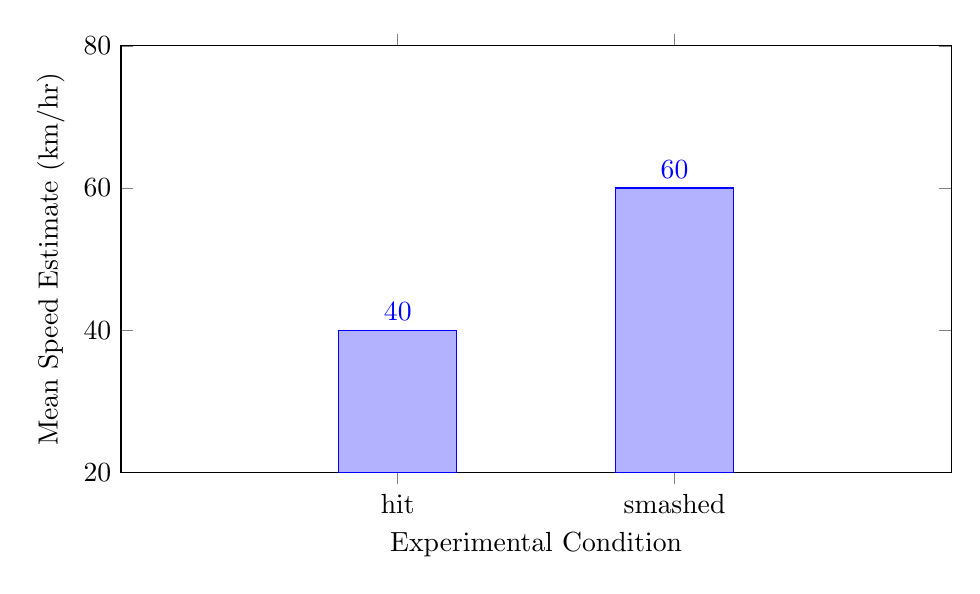
\begin{tikzpicture}
    \begin{axis}[
        ybar,
        width={\columnwidth},
        height=7cm,
        ylabel={Mean Speed Estimate (km/hr)},
        xlabel={Experimental Condition},
        symbolic x coords={hit,smashed},
        enlargelimits=1.0,
        bar width=1.5cm,
        xtick=data,
        nodes near coords,
        nodes near coords align={vertical},
        x tick label style={anchor=north}]
    \addplot coordinates {(hit, 40) (smashed,60)};
    \end{axis}
\end{tikzpicture}
\end{center}
\caption{Comparison of mean speed estimates.}
\end{figure}

The results clearly show a difference between the speed estimates in the
two experimental conditions. The mean speed estimates in the “smashed”
condition are 50\% higher than the mean speed estimates in the “hit”
condition.

See the Appendix, subsection 2 for the raw data and calculations.

\section{Discussion}

The result of our experiment clearly suggest that the use of leading
questions does indeed influence memory. As in the original study conducted
by Loftus and Palmer, the mean speed estimate was significantly higher in
the “smashed” condition than in the “hit” condition. Based on the
reconstructive theory of memory proposed by Bartlett, these results could
be explained due to the triggering of the schemata associated with the
respective verbs “smashed” and “hit”. The intense, dramatic schema
associated with the word “smashed” elicited higher speed estimates, while
the milder, less intense schema associate with the word “hit” elicited
lower speed estimates.

In conclusion, extra information obtained from the schemata associated with
the verb in the leading question interfered with the retrieval of memory,
causing differing mean speed estimates in the two experimental conditions.
This conclusion closely resembles that of Loftus and Palmer, who also
showed that the schema associated with the verb used in the leading question
interfered with memory retrieval.

Despite the solid conclusions we were able to draw, this experiment suffers
from several limitation both in it’s design and it’s procedure. Firstly,
the extremely small sample size and the use of opportunity sampling
introduced significant bias to the results, as not every stratum of the
population was represented. Furthermore, although a double blind design was
used, the experimenter (due to the sampling method used) may have
inadvertently chosen participants who were more likely to give answers he
expected or wanted. As in the original study, the experiment lacked
ecological validity, as participants were shown a video of a car crash
rather than the real thing. In the real life event, they might have been
able to assimilate more information about the crash, perhaps even enough
information to disregard the extra information communicated in the leading
question. Furthermore, the quality of the video of the car crash was far
less than ideal; unlike our eyes and ears, the image wasn’t very high
resolution and the sound was fair. Therefore, the net information
communicated in the video was far less than what would have been
communicated in real life. Lastly, the experiment does not directly
address the fact that these verbs have interfered with the recall of the
memory of the car crash, rather, it only shows that these verbs interfered
with the recall of the speed at which the crash occurred. To ascertain
whether the real memory of the crash were affected, I would have to test
whether other elements likely to be associated with the verb’s schema were
present in the participants’ memories. Otherwise, it could be argued that
the extra information communicated in the leading question helped the
participant choose a more accurate speed, and no memory was really altered.
In the original study conducted by Loftus and Palmer, a second experiment
was used to establish the fact that the memory was truly modified.

Conducting this experiment over, I would definitely expand the sample
population and use a less biased sampling method, such as random sampling.
This would reduce the bias introduced by the small population and allow the
findings of the study to easily generalize. The ecological validity of the
experiment could also be improved by attempting to use real life car
accidents and accident witnesses, however, this remains difficult and
dangerous.

\bibliographystyle{plain}
\bibliography{doc.bib}

\clearpage
\section{Appendix}

\subsection{Materials and Apparatus}

\begin{figure}[h]
\begin{center}
\begin{tabular}{cc}
\toprule
Item & URL\\
\midrule
Consent form & \url{http://bit.ly/VKofDc}\\
Debriefing form & \url{http://bit.ly/YHO7gc}\\
Video of car crash & \url{http://bit.ly/11Rrb2O}\\
Questionnaires & \url{http://bit.ly/Xrwn5T}\\
\bottomrule
\end{tabular}
\end{center}
\caption{URL locations of the materials used in this study.}
\end{figure}

\subsection{Raw Data and Calculations}

\begin{figure}[h]
\begin{center}
\begin{tabular}{ccc}
\toprule
Participant & Speed Estimate & Condition\\
\midrule
1 & 50 & hit\\
2 & 40 & hit\\
3 & 30 & hit\\
4 & 40 & hit\\
5 & 70 & smashed\\
6 & 90 & smashed\\
7 & 40 & smashed\\
8 & 50 & smashed\\
9 & 60 & smashed\\
10& 50 & smashed\\
\bottomrule
\end{tabular}
\end{center}
\caption{Raw data of both experimental conditions.}
\end{figure}

The mean for both experimental conditions was calculated using the following
formula,
\begin{align*}
    \mu = \frac{1}{n}\sum{x}.\\
\end{align*}
Therefore,
\begin{align*}
    \mu_{\text{hit}} &= \frac{1}{4}\sum{x}\\
    &= \frac{1}{4} \cdot 160\\
    &= 40.
\end{align*}
And,
\begin{align*}
    \mu_{\text{smashed}} &= \frac{1}{6}\sum{x}\\
    &= \frac{1}{6} \cdot 360\\
    &= 60.
\end{align*}

The range for both experimental conditions was calculated using the following
formula,
\begin{align*}
    \text{range} = \max{x} - \min{x}.
\end{align*}
Therefore,
\begin{align*}
    \text{range}_{\text{hit}} &= \max{x} - \min{x}\\
    &= 50 - 30\\
    &= 20.
\end{align*}
And,
\begin{align*}
    \text{range}_{\text{smashed}} &= \max{x} - \min{x}\\
    &= 90 - 40\\
    &= 50.
\end{align*}

\end{document}
